\documentclass[12pt]{article} % use larger type; default would be 10pt
\usepackage[utf8]{inputenc} % set input encoding (not needed with XeLaTeX)

%%% PAGE DIMENSIONS
\usepackage{geometry} % to change the page dimensions
\geometry{a4paper} % or letterpaper (US) or a5paper or....
\geometry{margin=2cm} % or letterpaper (US) or a5paper or....

\usepackage{graphicx} % support the \includegraphics command and options
\usepackage[parfill]{parskip} % Activate to begin paragraphs with an empty line rather than an indent
\usepackage{times} % for Times Roman default font

%%% PACKAGES
\usepackage{booktabs} % for much better looking tables
\usepackage{array} % for better arrays (eg matrices) in maths
\usepackage{paralist} % very flexible & customisable lists (eg. enumerate/itemize, etc.)
\usepackage{verbatim} % adds environment for commenting out blocks of text & for better verbatim
\usepackage{subfig} % make it possible to include more than one captioned figure/table in a single float

%%% HEADERS & FOOTERS
\usepackage{fancyhdr} % This should be set AFTER setting up the page geometry
\pagestyle{fancy} % options: empty , plain , fancy
\renewcommand{\headrulewidth}{0pt} % customise the layout...
\lhead{}\chead{}\rhead{}
\lfoot{}\cfoot{\thepage}\rfoot{}

\makeatletter
\renewcommand{\maketitle}{%
  {\bfseries{\scshape{\Large{\@title\par}}}}
}
\makeatother

\hyphenation{Kiwi-bank} % otherwise it may get hyphenated as Ki-wibank

%%% END Article customizations

%%% The "real" document content comes below...

\title{Lucretia Biv: 14-15 May 2017}

\begin{document}
  \maketitle
We undertook this trip as we had heard via Permolat that DoC are looking for someone to take over maintenance of this wee biv.  The walk into the biv was relatively straight-forward.  Unfortunately, as I am writing this about a week after the event, I cannot remember the walking times accurately.  I do recall that we comfortably bettered the track time by about half an hour which \textit{I think} means we had about 4.5 hours walking to the biv.  I do know we had an early lunch when we got to Lucretia Stream.  The track up the Lucretia is less travelled and not quite so easy to follow (in fact, we got a little confused shortly after starting up the stream by an apparent track leading upwards, whereas the actual track went onto the open grassy clearings on the creek bed).  There is one crossing of Lucretia about half way up.  Since it was pretty cold we elected to take our boots off for this and thus keep dry socks.

There was a lot of recent windfall around the biv which would have offered ample firewood had it been a bit drier.  Nevertheless we managed to collect sufficient dry-ish fuel to get the fire going and after some diligent effort obtained a bed of embers with enough heat to keep it going.  It was a pretty cold night.  Robyn slept - well lay down anyway - with the dog in her bag for mutual warmth, but my bag is warmer so I was quite cosy.  In the morning we made some notes and measurements regarding the maintenance, and then headed off upstream.

\begin{figure}[ht]
%\centering
\begin{minipage}{.45\linewidth}
\begin{flushleft}
   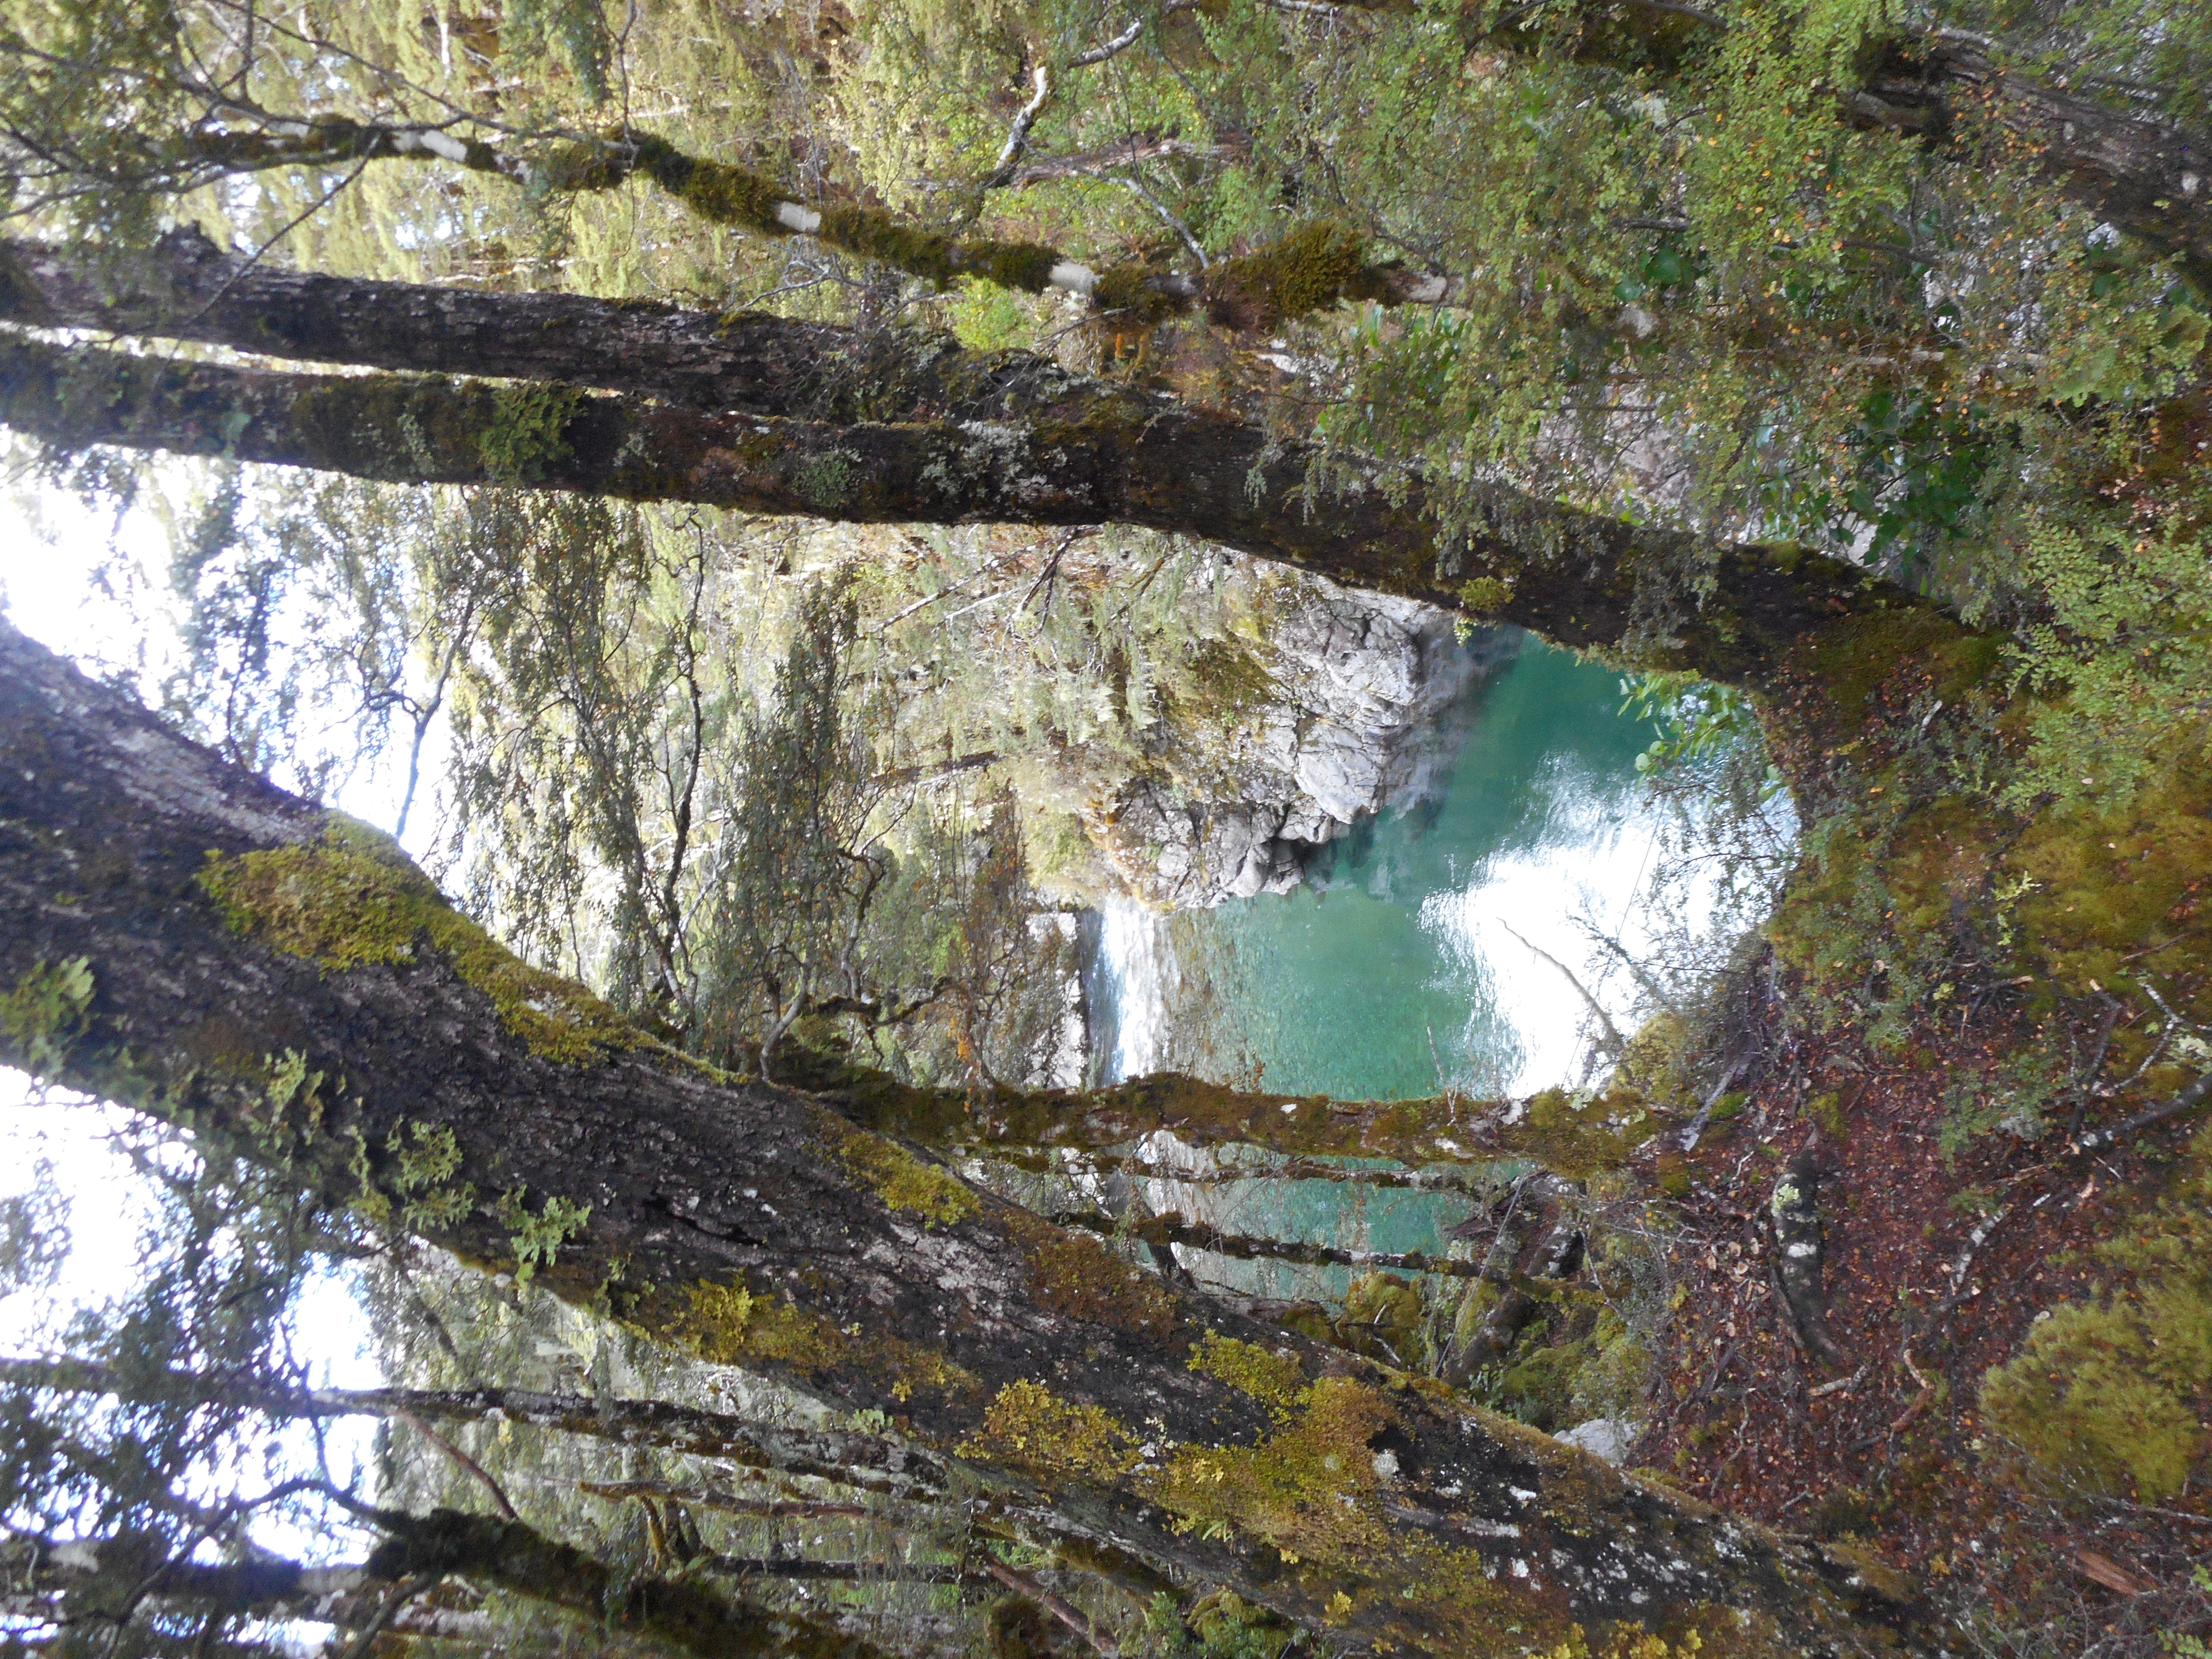
\includegraphics[width=10cm, angle=270]{LucretiaBiv14May2017Photo1}
\end{flushleft}
\end{minipage}
\begin{minipage}{.55\linewidth}
\begin{flushright}
    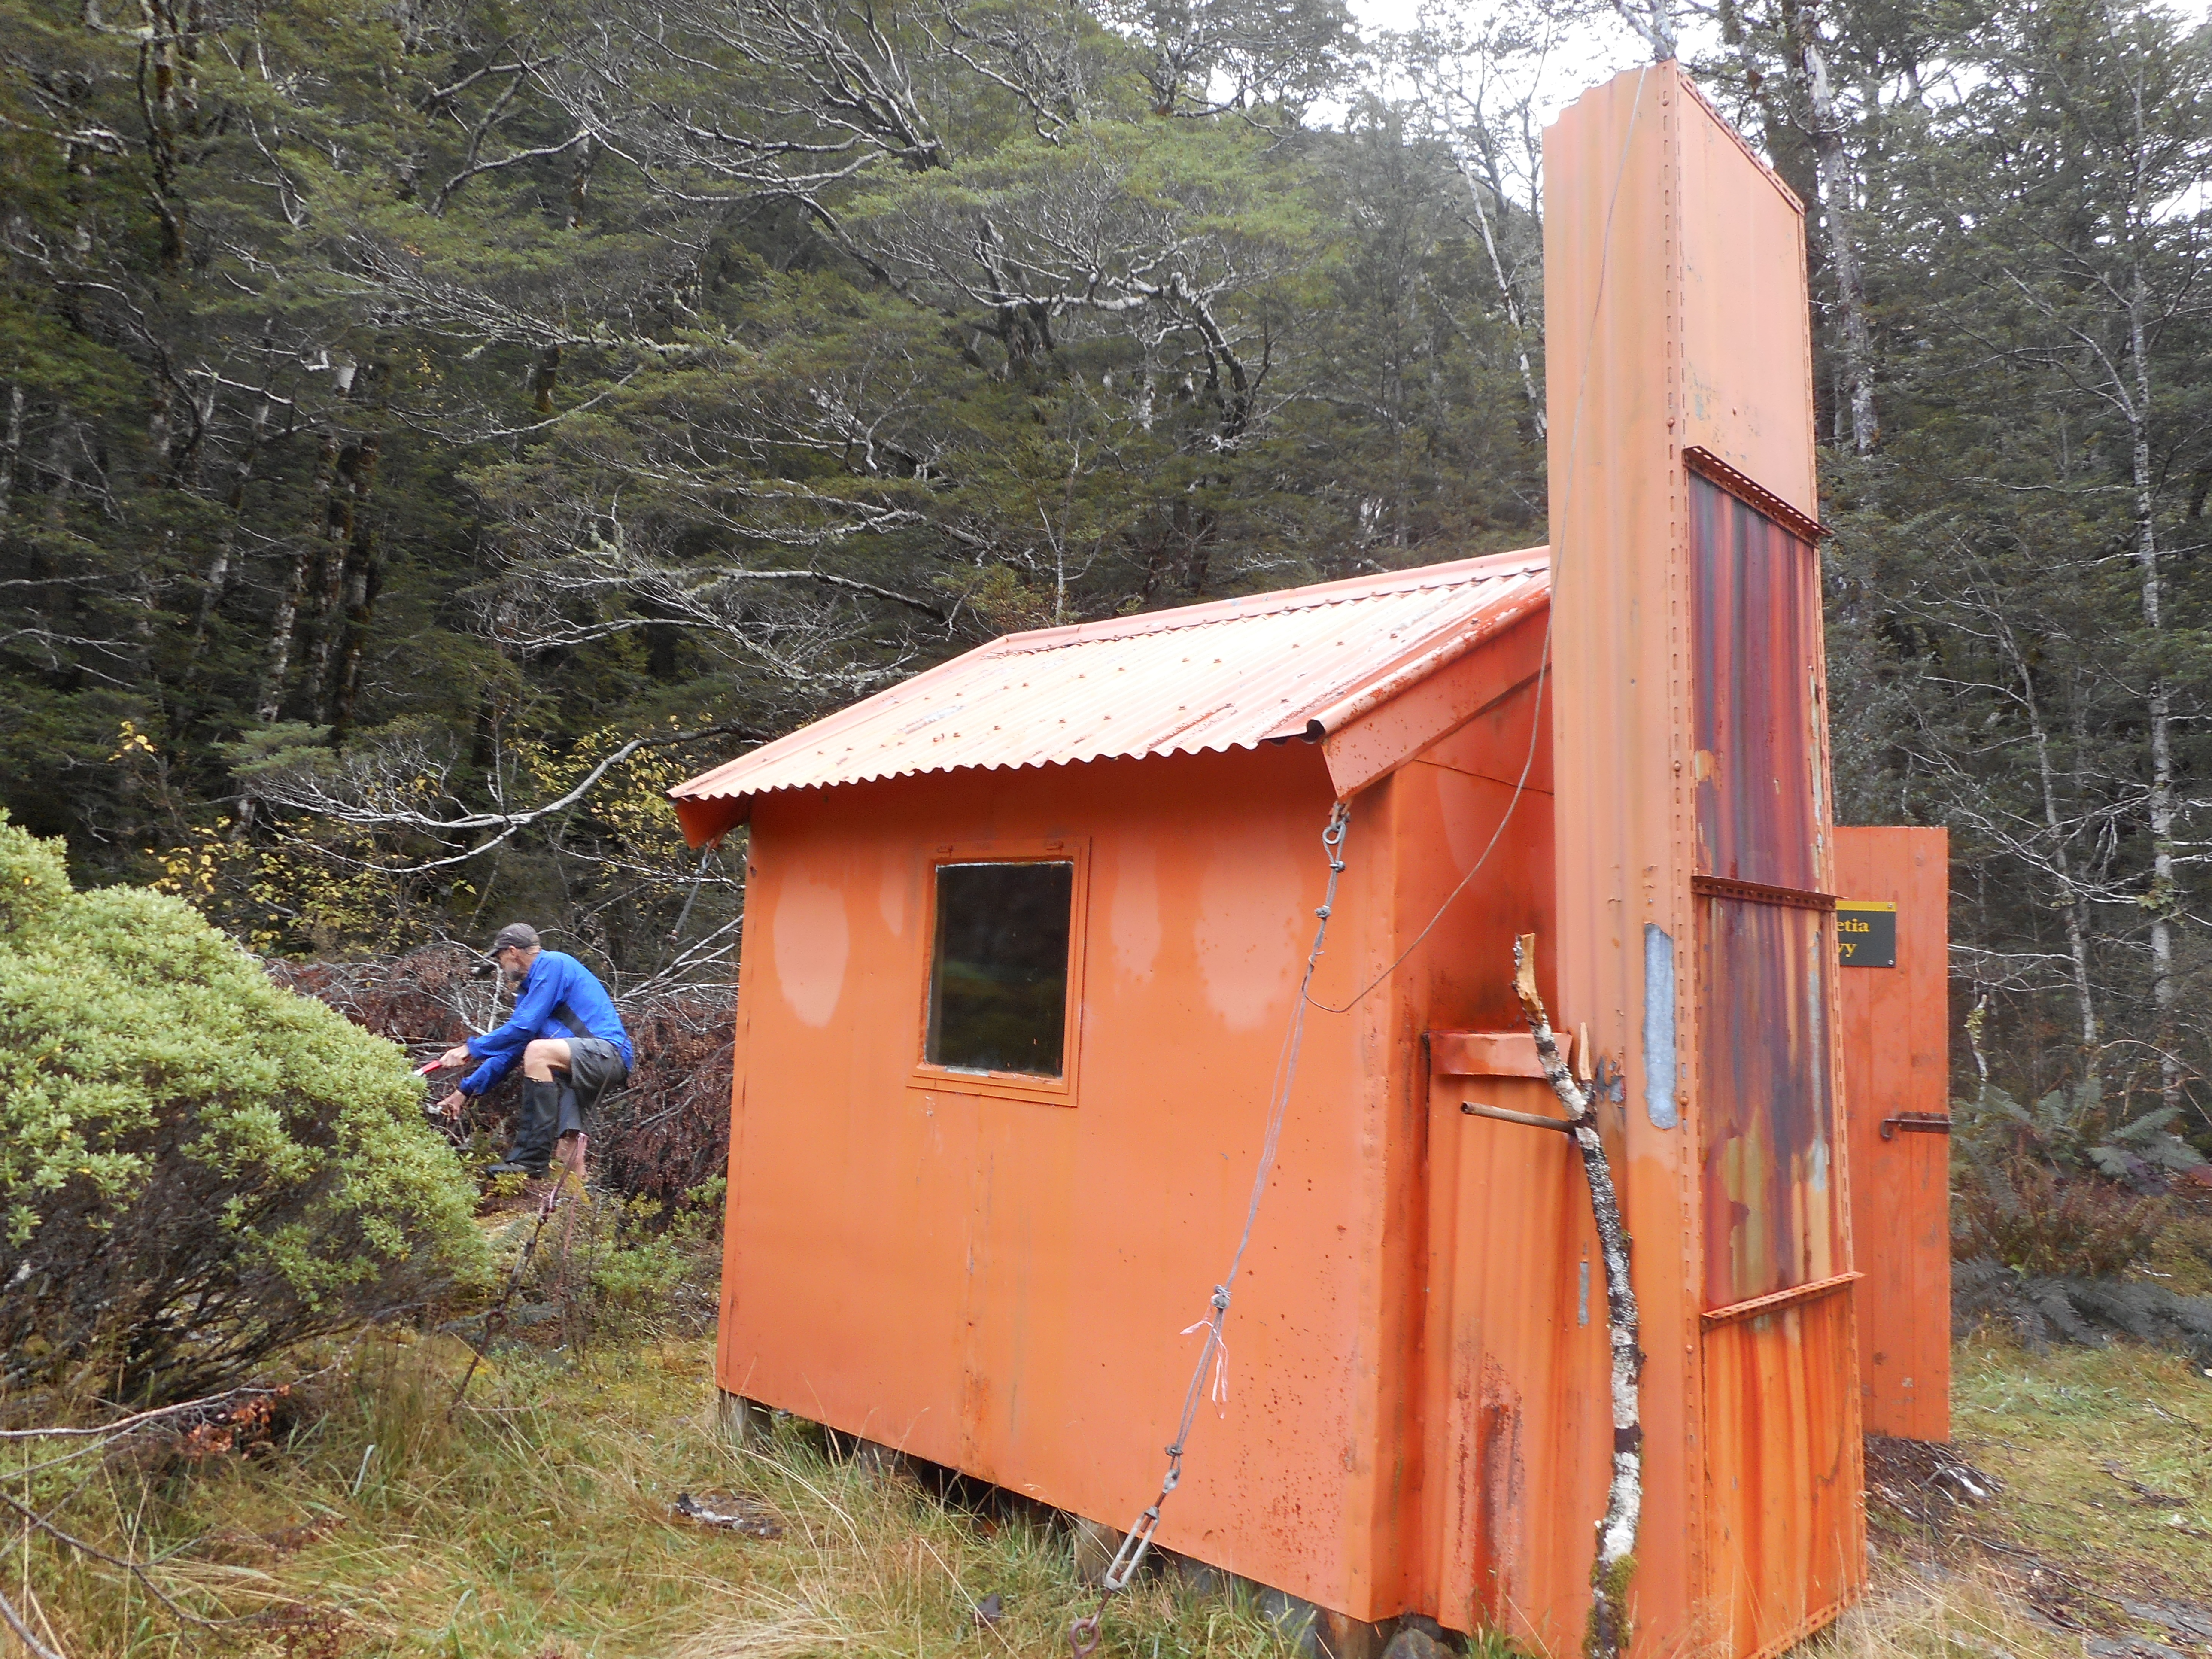
\includegraphics[width=10cm]{LucretiaBiv14May2017Photo2}
\end{flushright}
\end{minipage}
\end{figure}

There is (or was then) a marked track up to the third stream coming in on Lucretia's true right (i.e., our left going up), and then onto the tops via the spur beyond.  It would have been shorter heading up beside the Lucretia waterfall (probably true left) above the bushline and hence to the saddle with the tarns.  However, being the first time up we stuck to the track, and given the frost this was probably not such a bad decision as the head of Lucretia Stream is pretty steep and was in the shade all day (and hence the frost didn't thaw).  As it was we had to scramble over Lucretia itself which was a bit nerve-racking when we had to skirt round on the frosty side.  However, we managed without mishap and had a late lunch just above the saddle between Lucretia and the Apprentice.

After lunch, Robyn and I parted as I thought it would be easier to cut across from the Lucretia-Apprentice saddle to the Technical-Apprentice saddle and head NNE to get to high-point 1580 at the end of the Lewis Tops.  Robyn preferred to go over the Apprentice as we had done that before.  In retrospect, we agreed that the way I took was easier.

From high point 1580, which we reached at 14:30 (actually I first reached it before 14:00), we separated again as I wished to stride ahead in order to hitch-hike back to Palmer lodge for the car before dusk.  I made it to the top of the pass by 16:00 (i.e., an hour and half), and then had to wait for about half an hour before a farmer from Ellesmere gave me a ride in his truck.  Robyn arrived about 15 minutes after this so had a bit of a wait before I returned with the car.

This is a great two-day hike, albeit a little cold in May.

\begin{flushright}
Robyn, Peter and dog
\end{flushright}

\end{document}
